% This document is used for Daya Bay MACRO PMT pressure test report


\documentclass{beamer}
\usepackage{graphicx}

\usepackage{ragged2e}
\justifying

\usepackage{setspace}

\setbeamertemplate{navigation symbols}{}
\setbeamertemplate{footline}[page number]
\setbeamertemplate{caption}[numbered]

\usetheme{default}
\logo{
\includegraphics[height=1cm]{Dyb_logo.png}}
\begin{document}
\title{Status of MACRO PMT pressure tests at SAB}
\author{Logan Lebanowski, Shih-Kai Lin}
%\institute{University of Houston}
\date{2010 October 7}

\begin{frame}
\begin{center}
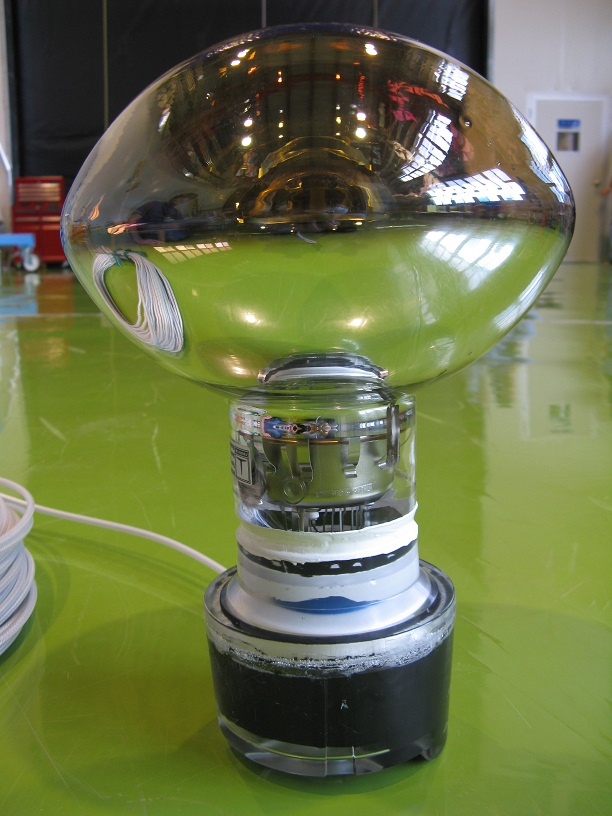
\includegraphics[height=4cm]{IMG_1048.jpg}
\end{center}
\titlepage
\end{frame}


\begin{frame}{overview}
	\begin{itemize}
		\item 150 waterproof MACRO EMI PMT assemblies need to be pressure tested
			at the SAB. They have already passed performance tests at DGUT.
		\item We test about 10 PMTs per week (mid-August to December).
		\item For more information, see
			\textcolor{blue}{\href
			{http://dayabay.ihep.ac.cn/cgi-bin/DocDB/ShowDocument?docid=5373}{doc 5373}}.
	\end{itemize}
		\begin{center}
			\underline{As of October 7, we have passed 60 of 68 tested PMTs.}
		\end{center}
	\begin{center}
		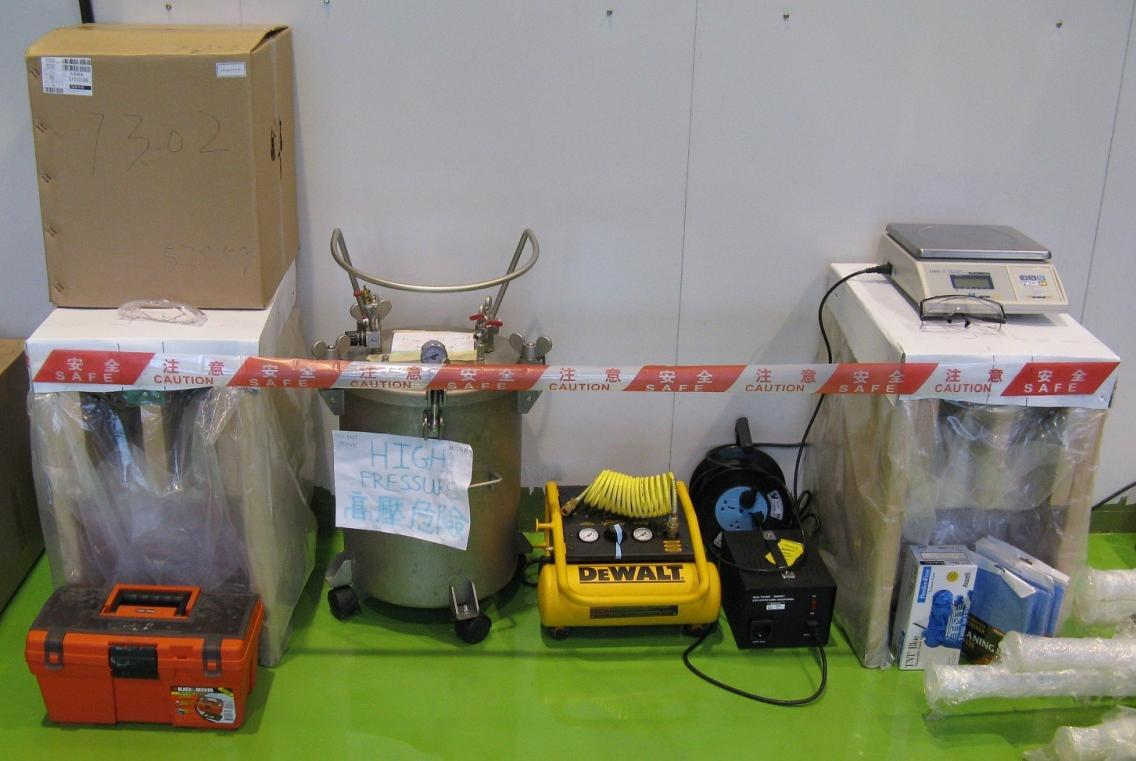
\includegraphics[height=4cm]{test_setup.jpeg}
	\end{center}
\end{frame}


\begin{frame}{pressure test results}
	\begin{center}
		\small
		8 PMTs were tested during the past week (September 30 - October 6).
	\end{center}
\begin{table}
\small
\setstretch{0.4}
\begin{tabular}{c|c|c|c|c}
%\setlength{\tabcolsep}{2pt}
	SN & mass (g) & pressure (psig) & test time (h:m) & result \\
	\hline
	6502 & 590.5 & 12.0 & 14:45 & PASS$^1$ \\
	7117 & 600 & 12.2 & 8:22 & PASS$^1$ \\
	{\color{green}8727}$^\dagger$ & {\color{green}574} & {\color{green}12.1}
	& {\color{red}87:02} & {\color{green}NOT PASS}$^3$ \\
	8819 & 582.5 & 12.1 & 7:51 & PASS$^1$ \\
	6380 & 616.5 & 12.7 & 15:39 & PASS$^2$ \\
	7925 & 571 & 12.1 & 8:07 & PASS$^1$ \\
	7525 & 630 & 12.1 & 14:43 & PASS$^1$ \\
	6796 & 573 & 12.1 & 8:33 & PASS$^1$ \\
\end{tabular}
%\caption {pressure test result: For PASS/FAIL reasons, please see the table in the next slide.}
\end{table}
	\setstretch{0.1}
	\scriptsize
	$^\dagger$ A hole was found in the jacket of the cable on September 23. It was then 
	repaired with mastic tape and heat shrink tubing and pressure tested again on September 30.
%\begin{itemize}
%	\item For PASS/FAIL reasons, please see the table in the next slide.
%\end{itemize}
	\setlength{\tabcolsep}{2pt}
	\scriptsize
	\begin{table}
		\begin{tabular}{|c|p{3.5in}|}
		\hline
		1 & Cable dry. No leaks or cracks. \\
		\hline
		2 & 1+Some water penetrated the mastic tape seal of the cable strain relief plug,
			but did not penetrate the UW cable plug. \\
		\hline
		3 & Cable sealing tube still had some water. The way the cable was repaired didn't
		work well.\\
		\hline
		\end{tabular}
	%\caption{PASS/FAIL reasons}
	\end{table}
\end{frame}


\begin{frame}{signal test results}
	\setstretch{0.3}
	\small The operational capability of a PMT is verified after pressure testing:\\
	{\scriptsize The PMT is placed in a dark box, connected to a single channel decoupler box,
	and set to its 2E7 gain voltage, as recorded in the DGUT data. After tens of minutes,
	the count rate, rise time, and pulse height are recorded. We use a threshold of 3.00 
	mV, which is roughly 1/4 pe.
	}

	\setstretch{1}
	\setlength{\tabcolsep}{2pt}
	\small
	\begin{center}
	\begin{tabular}{|l|p{1.2cm}|p{1.9cm}|p{1.5cm}|p{1.7cm}|}
		\hline
		\textbf{SN}&\textbf{Rate (kHz)}&\textbf{DGUT rate (kHz)}&\textbf{Rise time (ns)}&
		\textbf{DGUT rise time (ns)}\\
		\hline
		\hline
		6340&9.0&1.62&4.1&3.8\\
		6347&7.0&2.04&4.6&4.6\\
		8866&5.0&1.49&5.1&5.5\\
		8700&1.5&0.43&5.2&7.5\\
		6502&3.0&1.81&5.5&7.1\\
		7117&5.0&3.36&4.6&5.4\\
		\hline
	\end{tabular}
		\begin{itemize}
			\item Rates are all below 10 kHz.
		\end{itemize}
	\end{center}
\end{frame}


\end{document}

